\documentclass[a4paper,14pt]{extarticle}

\usepackage[utf8x]{inputenc}
\usepackage[T1,T2A]{fontenc}
\usepackage[russian]{babel}
\usepackage{hyperref}
\usepackage{indentfirst}
\usepackage{here}
\usepackage{array}
\usepackage{graphicx}
\usepackage{caption}
\usepackage{subcaption}
\usepackage{chngcntr}
\usepackage{amsmath}
\usepackage{amssymb}
\usepackage{amsthm}
\usepackage{pgfplots}
\usepackage{pgfplotstable}
\usepackage[left=2cm,right=2cm,top=2cm,bottom=2cm,bindingoffset=0cm]{geometry}
\usepackage{multicol}
\usepackage{askmaps}
\usepackage{titlesec}
\usepackage{listings}
\usepackage{color}
\usepackage{enumerate}
\usepackage{hhline}
\usepackage{enumitem}
\usepackage{courier}
\usepackage{wrapfig}
\usetikzlibrary{arrows,automata}

\setitemize{itemsep=0em}
\setenumerate{itemsep=0em}

\theoremstyle{definition}

\pgfkeys{/pgf/number format/.cd,1000 sep={\,}}

\definecolor{green}{rgb}{0,0.6,0}
\definecolor{gray}{rgb}{0.5,0.5,0.5}
\definecolor{purple}{rgb}{0.58,0,0.82}

\lstset{
	language=python,
	backgroundcolor=\color{white},   
	commentstyle=\color{green},
	keywordstyle=\color{blue},
	numberstyle=\tiny\color{gray},
	stringstyle=\color{purple},
	basicstyle=\footnotesize\ttfamily,
	breakatwhitespace=false,
	breaklines=true,
	captionpos=b,
	keepspaces=true,
	numbers=left,
	numbersep=5pt,
	showspaces=false,
	showstringspaces=false,
	showtabs=false,
	tabsize=2,
	frame=single,
	inputpath={../code/}
}

\renewcommand{\le}{\ensuremath{\leqslant}}
\renewcommand{\leq}{\ensuremath{\leqslant}}
\renewcommand{\ge}{\ensuremath{\geqslant}}
\renewcommand{\geq}{\ensuremath{\geqslant}}
\renewcommand{\epsilon}{\ensuremath{\varepsilon}}
\renewcommand{\phi}{\ensuremath{\varphi}}
\renewcommand{\thefigure}{\arabic{figure}} 	
\newcommand{\norm}[1]{\left\lVert#1\right\rVert}
\newcommand*\sfrac[2]{{}^{#1}\!/_{#2}}

%\titleformat*{\section}{\large\bfseries} 
\titleformat*{\subsection}{\normalsize\bfseries} 
\titleformat*{\subsubsection}{\normalsize\bfseries} 
\titleformat*{\paragraph}{\normalsize\bfseries} 
\titleformat*{\subparagraph}{\normalsize\bfseries} 

\counterwithin{figure}{section}
\counterwithin{equation}{section}
\counterwithin{table}{section}
\newcommand{\sign}[1][5cm]{\makebox[#1]{\hrulefill}}
\graphicspath{{../pics/}}
\captionsetup{justification=centering,margin=1cm}
\setlength\parindent{5ex}
\def\arraystretch{1.3}
\def\tabcolsep{12pt}
%\titlelabel{\thetitle.\quad}

\DeclareMathOperator*{\argmin}{argmin}
\DeclareMathOperator*{\argmax}{argmax}

\begin{document}

\begin{titlepage}
\begin{center}
	\textbf{Санкт-Петербургский Политехнический Университет \\Петра Великого}\\[0.3cm]
	\small Институт компьютерных наук и технологий \\[0.3cm]
	\small Кафедра компьютерных систем и программных технологий\\[4cm]
	
	\textbf{ОТЧЕТ}\\ \textbf{по расчетному заданию}\\[0.5cm]
	\textbf{<<Построение моделей>>}\\[0.1cm]
	\textbf{Системный анализ и принятие решений}\\[8.0cm]
\end{center}

\begin{flushright}
	\begin{minipage}{0.4\textwidth}
		\begin{flushleft}
			\small \textbf{Работу выполнил студент}\\[3mm]
			\small группа 33501/4 \hspace*{6mm} Дьячков В.В.\\[5mm]
			
			\small \textbf{Преподаватель}\\[5mm]
		 	\small \sign[3cm] \hspace*{5mm} Сабонис С.С.\\[0.5cm]
		\end{flushleft}
	\end{minipage}
\end{flushright}

\vfill

\begin{center}
	\small Санкт-Петербург\\
	\small \the\year
\end{center}
\end{titlepage}

\addtocounter{page}{1}

\section{Техническое задание}

\begin{enumerate}
	\setlength{\itemsep}{0.5em}
	\item Привести задачу к канонической форме;
	\item Решить задачу геометрическим методом;
	\item Обозначить все опорные точки (в том числе недопустимые) и записать соответствующие им наборы базисных переменных, рассчитать значение целевой функции в каждой опорной точке (решить задачу методом полного перебора опорных точек);
	\item Решить задачу симплекс-методом в матричной форме;
	\item Решить задачу симплекс-методом в табличной форме;
	\item Ввести дополнительное ограничение, отсекающее оптимальную точку. Решить новую задачу двойственным симплекс-методом в табличной форме, в качестве начального базиса новой задачи использовать оптимальный базис исходной задачи;
	\item Сформулировать задачу, двойственную по отношению к исходной. 
\end{enumerate}

\section{Исходные данные}

\paragraph{Вариант 32}

Дана задача линейного программирования:
\begin{equation}
\label{eq:main}
\begin{cases}
	\max \left( 2 x_1 + 3 x_2 \right) \\
	x_1 + x_2 \le 4.8 \\
	-3 x_1 - x_2 \le -3.5 \\
	x_1 \ge 0 \\
	x_2 \ge 0
\end{cases}
\end{equation}

\section{Приведение к канонической форме}

Приведём задачу к канонической форме при помощи введения новых переменных $x_3$ и $x_4$ и домножения второго ограничения на $-1$:

\begin{equation}
\begin{cases}
	\max \left( 2 x_1 + 3 x_2 \right) \\
	x_1 + x_2 + x_3 = 4.8 \\
	3 x_1 + x_2 - x_4 = 3.5 \\
	x_i \ge 0, i = \overline{1,4}
\end{cases}
\end{equation}

\section{Решение геометрическим методом}

На рис. \ref{pic:geometric_solution} изображено геометрическое представление системы \ref{eq:main}.

\begin{figure}[H]
\begin{center}
	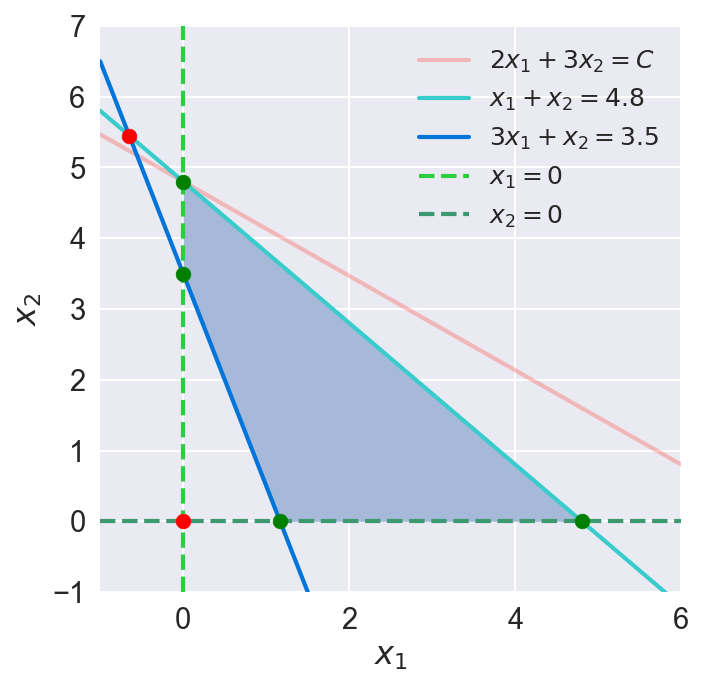
\includegraphics[scale=1]{system_1}
	\caption{Решение геометрическим методом}
	\label{pic:geometric_solution}
\end{center}
\end{figure}

Полученный выпуклый 4-угольник является областью допустимых решений. Зелеными точками на рисунке изображены допустимые опорные точки, красными -- недопустимые. Можно заметить, что максимальное значение в области допустимых значений прямая $2x_1 + 3x_2 = C$ принимает в точке $x_1 = 0$, $x_2 = 4.8$, следовательно эта опорная точка и является единственным решением задачи.

\section{Решение методом полного перебора опорных точек}

\begin{enumerate}[leftmargin=*]
\item 
	\label{eq:bad_basis_1}
	$\begin{cases}
		x_1 + x_2 = 4.8 \\
		3x_1 + x_2 = 3.5
	\end{cases}
	\Rightarrow
	\begin{cases}
		x_2 = 4.8 - x_1 \\
		2x_1 + 4.8 = 3.5
	\end{cases}
	\Rightarrow
	\begin{cases}
		x_1 = -0.65 \\
		x_2 = 5.45
	\end{cases}
	\Rightarrow
	f = 15.05$
	
\item
	\label{eq:opt_basis}
	$\begin{cases}
		x_1 + x_2 = 4.8 \\
		x_1 = 0
	\end{cases}
	\Rightarrow
	\begin{cases}
		x_1 = 0 \\
		x_2 = 4.8
	\end{cases}
	\Rightarrow
	f = 14.4$
	
\item
	$\begin{cases}
		x_1 + x_2 = 4.8 \\
		x_2 = 0
	\end{cases}
	\Rightarrow
	\begin{cases}
		x_1 = 4.8 \\
		x_2 = 0
	\end{cases}
	\Rightarrow
	f = 9.6$
	
\item
	$\begin{cases}
		3x_1 + x_2 = 3.5 \\
		x_1 = 0
	\end{cases}
	\Rightarrow
	\begin{cases}
		x_1 = 0 \\
		x_2 = 3.5
	\end{cases}
	\Rightarrow
	f = 10.5$
	
\item
	$\begin{cases}
		3x_1 + x_2 = 3.5 \\
		x_2 = 0
	\end{cases}
	\Rightarrow
	\begin{cases}
		x_1 = \frac{3.5}{3} \approx 1.17 \\
		x_2 = 0
	\end{cases}
	\Rightarrow
	f \approx 2.34$
	
\item 
	\label{eq:bad_basis_2}
	$\begin{cases}
		x_1 = 0 \\
		x_2 = 0
	\end{cases}
	\Rightarrow
	f = 0$
\end{enumerate}

При проверке найденных опорных точек на допустимость в системе уравнений \ref{eq:main} видно, что точки \ref{eq:bad_basis_1} и \ref{eq:bad_basis_2} являются недопустимыми. Максимальное значение функция принимает в точке \ref{eq:bad_basis_1}, но так как данная точка является недопустимой, оптимальной точкой является точка \ref{eq:opt_basis} ($x_1 = 0, x_2 = 4.8$).

\section{Решение симплекс-методом в матричной форме}

Запишем матрицу коэффициентов системы \ref{eq:main}:
\begin{equation*}
A = 
\begin{pmatrix}
	1 & 1 & 1 & 0 \\
	3 & 1 & 0 & -1
\end{pmatrix}
\end{equation*}

Из данной матрицы невозможно выделить единичную подматрицу, поэтому введем переменную $x_5$. Тогда система приобретает следующий вид:

\begin{equation}
\label{eq:canonic}
\begin{cases}
	\max \left( 2 x_1 + 3 x_2 \right) \\
	x_1 + x_2 + x_3 = 4.8 \\
	3 x_1 + x_2 - x_4 + x_5 = 3.5 \\
	x_i \ge 0, i = \overline{1,5}
\end{cases}
\end{equation}

Перепишем систему \ref{eq:canonic} в матричной форме:
\begin{equation*}
A = 
\begin{pmatrix}
	1 & 1 & 1 & 0 & 0\\
	3 & 1 & 0 & -1 & 1
\end{pmatrix},\text{ }
b = 
\begin{pmatrix}
	4.8 \\
	-3.5
\end{pmatrix},\text{ }
c = 
\begin{pmatrix}
	2 & 3 & 0 & 0 & 0
\end{pmatrix}^T,\text{ }
x = 
\begin{pmatrix}
	x_1 & \cdots & x_5 
\end{pmatrix}^T
\end{equation*}

\begin{equation}
\begin{cases}
	\max (c^Tx) \\
	A x = b \\
	b \ge 0 \\
	x \ge 0
\end{cases}
\end{equation}

Переменные $x_3$ и $x_5$ формируют единичную подматрицу $P = \left( \begin{smallmatrix} 1 & 0 \\ 0 & 1 \end{smallmatrix} \right)$ в матрице $A$, следовательно выберем их как базисные переменные, а $x_1$, $x_2$ и $x_4$ как свободные переменные.

\begin{enumerate}[leftmargin=*]

\item
$x^\text{Б} = P^{-1}b =
\begin{pmatrix}
	1 & 0 \\
	0 & 1 
\end{pmatrix}
\begin{pmatrix}
	4.8 \\
	3.5
\end{pmatrix} =
\begin{pmatrix}
	4.8 \\
	3.5
\end{pmatrix} \geq 0
\Rightarrow$ базис допустим.

$c^\text{Б} = 
\begin{pmatrix}
	0 & 0
\end{pmatrix}$

Для свободных переменных найдем $\Delta_i$ ($i = 1, 2, 4$):

$\Delta_1 = c^\text{Б} P^{-1} A_1 - c_1 =
\begin{pmatrix}
	0 & 0
\end{pmatrix}
\begin{pmatrix}
	1 & 0 \\
	0 & 1 
\end{pmatrix}
\begin{pmatrix}
	1 \\
	3
\end{pmatrix} - 2 = -2$

$\Delta_2 = c^\text{Б} P^{-1} A_2 - c_2 =
\begin{pmatrix}
	0 & 0
\end{pmatrix}
\begin{pmatrix}
	1 & 0 \\
	0 & 1 
\end{pmatrix}
\begin{pmatrix}
	1 \\
	1
\end{pmatrix} - 3 = -3$

$\Delta_4 = c^\text{Б} P^{-1} A_4 - c_4 =
\begin{pmatrix}
	0 & 0
\end{pmatrix}
\begin{pmatrix}
	1 & 0 \\
	0 & 1 
\end{pmatrix}
\begin{pmatrix}
	0 \\
	-1
\end{pmatrix} - 0 = 0$

$\Delta = \begin{pmatrix} -2 & -3 & 0 \end{pmatrix}^T \ngeqslant 0 \Rightarrow$ базис не оптимален. 

Вводим в базис переменную $x_k$, т.ч. $k = \argmin\limits_i\Delta_i = 2 \Rightarrow x_2$.

Определим вектор $z = P^{-1} A_k = P^{-1} A_2 = 
\begin{pmatrix}
	1 & 0 \\
	0 & 1 
\end{pmatrix}
\begin{pmatrix}
	1 \\
	1
\end{pmatrix} =
\begin{pmatrix}
	1 \\
	1
\end{pmatrix}$.

Выводим из базиса переменную $x_r$, т.ч. 
$r = \argmin\limits_j\left( \left. \dfrac{x_j^\text{Б}}{z_j}\right|_{z_j>0} \right) = 5 \Rightarrow x_5$.

\item 
Меняем местами $x_2$ и $x_5$, следовательно новый базис состоит из $x_2$ и $x_3$, а $x_1$, $x_4$ и $x_5$ -- свободные переменные. 

$P = 
\begin{pmatrix}
	1 & 1 \\
	1 & 0 
\end{pmatrix} \Rightarrow
P^{-1} = 
\begin{pmatrix}
	0 & 1 \\
	1 & -1 
\end{pmatrix}$

$x^\text{Б} = P^{-1}b =
\begin{pmatrix}
	0 & 1 \\
	1 & -1
\end{pmatrix}
\begin{pmatrix}
	4.8 \\
	3.5
\end{pmatrix} =
\begin{pmatrix}
	3.5 \\
	1.3
\end{pmatrix} \geq 0
\Rightarrow$ базис допустим.

$c^\text{Б} = 
\begin{pmatrix}
	3 & 0
\end{pmatrix}$

Для свободных переменных найдем $\Delta_i$ ($i = 1, 4, 5$):

$\Delta_1 = c^\text{Б} P^{-1} A_1 - c_1 =
\begin{pmatrix}
	3 & 0
\end{pmatrix}
\begin{pmatrix}
	0 & 1 \\
	1 & -1
\end{pmatrix}
\begin{pmatrix}
	1 \\
	3
\end{pmatrix} - 2 = 
9 - 2 = 7$

$\Delta_4 = c^\text{Б} P^{-1} A_4 - c_4 =
\begin{pmatrix}
	3 & 0
\end{pmatrix}
\begin{pmatrix}
	0 & 1 \\
	1 & -1
\end{pmatrix}
\begin{pmatrix}
	0 \\
	-1
\end{pmatrix} - 0 = -3 - 0 = -3$

$\Delta_5 = c^\text{Б} P^{-1} A_5 - c_5 =
\begin{pmatrix}
	3 & 0
\end{pmatrix}
\begin{pmatrix}
	0 & 1 \\
	1 & -1 
\end{pmatrix}
\begin{pmatrix}
	0 \\
	1
\end{pmatrix} - 0 = 3 - 0 = 3$

$\Delta = \begin{pmatrix} 7 & -3 & 3 \end{pmatrix}^T \ngeqslant 0 \Rightarrow$ базис не оптимален. 

Вводим в базис переменную $x_k$, т.ч. $k = \argmin\limits_i\Delta_i = 4 \Rightarrow x_4$.

Определим вектор $z = P^{-1} A_k = P^{-1} A_4 = 
\begin{pmatrix}
	0 & 1 \\
	1 & -1
\end{pmatrix}
\begin{pmatrix}
	0 \\
	-1
\end{pmatrix} =
\begin{pmatrix}
	-1 \\
	1
\end{pmatrix}$.

Выводим из базиса переменную $x_r$, т.ч. 
$r = \argmin\limits_j\left( \left. \dfrac{x_j^\text{Б}}{z_j}\right|_{z_j>0} \right) = 3 \Rightarrow x_3$.

\item 
Меняем местами $x_3$ и $x_4$, следовательно новый базис состоит из $x_2$ и $x_4$, а $x_1$, $x_3$ и $x_5$ -- свободные переменные.

$P = 
\begin{pmatrix}
	1 & 0 \\
	1 & -1
\end{pmatrix} \Rightarrow
P^{-1} = 
\begin{pmatrix}
	1 & 0 \\
	1 & -1
\end{pmatrix}$

$x^\text{Б} = P^{-1}b =
\begin{pmatrix}
	1 & 0 \\
	1 & -1
\end{pmatrix}
\begin{pmatrix}
	4.8 \\
	3.5
\end{pmatrix} =
\begin{pmatrix}
	4.8 \\
	1.3
\end{pmatrix} \geq 0
\Rightarrow$ базис допустим.

$c^\text{Б} = 
\begin{pmatrix}
	3 & 0
\end{pmatrix}$

Для свободных переменных найдем $\Delta_i$ ($i = 1, 3, 5$):

$\Delta_1 = c^\text{Б} P^{-1} A_1 - c_1 =
\begin{pmatrix}
	3 & 0
\end{pmatrix}
\begin{pmatrix}
	1 & 0 \\
	1 & -1
\end{pmatrix}
\begin{pmatrix}
	1 \\
	3
\end{pmatrix} - 2 = 3 - 2 = 1$

$\Delta_3 = c^\text{Б} P^{-1} A_3 - c_3 =
\begin{pmatrix}
	3 & 0
\end{pmatrix}
\begin{pmatrix}
	1 & 0 \\
	1 & -1
\end{pmatrix}
\begin{pmatrix}
	1 \\
	0
\end{pmatrix} - 0 = 3 - 0 = 3$

$\Delta_5 = c^\text{Б} P^{-1} A_5 - c_5 =
\begin{pmatrix}
	3 & 0
\end{pmatrix}
\begin{pmatrix}
	1 & 0 \\
	1 & -1
\end{pmatrix}
\begin{pmatrix}
	0 \\
	1
\end{pmatrix} - 0 = 0 - 0 = 0$

$\Delta = \begin{pmatrix} 1 & 3 & 0 \end{pmatrix}^T \geq 0 \Rightarrow$ базис оптимален. 

Следовательно точка $x^{opt} = \begin{pmatrix} 0 & 4.8 & 0 & 1.3 & 0 \end{pmatrix}$ является оптимальным решением, что соотносится с геометрическим решением $x_1 = 0$, $x_2 = 4.8$. Значение функции при этом равно $x^{opt} \cdot c = 14.4$.

\end{enumerate}

\newpage

\section{Решение симплекс-методом в табличной форме}

Переменные $x_3$ и $x_5$ составляют в матрице $A$ единичную подматрицу, следовательно выберем их как базисные переменные, значит $x_1$, $x_2$ и $x_4$ -- свободные переменные. Выразим через них базисные переменные:
\begin{equation*}
\begin{cases}
	\max \left( 2 x_1 + 3 x_2 \right) \\
	x_1 + x_2 + x_3 = 4.8 \\
	3 x_1 + x_2 - x_4 + x_5 = 3.5 \\
	x_i \ge 0, i = \overline{1,5}
\end{cases}
\Rightarrow
\begin{cases}
	x_3 = 4.8 - x_1 - x_2 \\
	x_5 = 3.5 - 3x_1 - x_2 + x_4
\end{cases}
\end{equation*}

В таблице \ref{tab:simplex_1} приведена таблица симплекс метода для первого базиса.

\begin{table}[H]
\begin{center}
	\def\tabcolsep{15pt}
	\def\arraystretch{1.3}
	\caption{Базис $x_3, x_5$}
	\label{tab:simplex_1}
	\begin{tabular}{|c||c|c|c||c|}
		\hline
		№1.1 & $x_1$ & $x_2$ & $x_4$ & $b$ \\ 
		\hhline{|=#===#=|}
		$x_3$ & $-1$ & $-1$ & $0$ & $4.8$ \\ 
		\hline
		$x_5$ & $-3$ & \textcolor{red}{\boldmath$-1$} & $1$ & $3.5$\\ 
		\hhline{|=#===#=|}
		$f$ & $2$ & $3$ & $0$& $0$ \\ 
		\hline
	\end{tabular}
\end{center}
\end{table}

Базис является допустимым, так как $b \geq 0$, но не является оптимальным, так как $c \nleqslant 0$. Выберем $x_2$ как разрешающий столбец, а $x_5$ как разрешающую строку. На их пересечении находится разрешающий элемент $-1$. В таблице \ref{tab:simplex_2} приведена промежуточная таблица симплекс метода, в которой поменяны местами $x_2$ и $x_5$ и базисными являются $x_2$ и $x_3$.

\begin{table}[H]
\begin{center}
	\def\tabcolsep{14pt}
	\def\arraystretch{1.3}
	\caption{Промежуточная таблица базиса $x_2, x_3$}
	\label{tab:simplex_2}
	\begin{tabular}{|c||c|c|c||c|}
		\hline
		№2.1 & $x_1$ & $x_5$ & $x_4$ & $b$ \\ 
		\hhline{|=#===#=|}
		$x_3$ & $-2$ & $-1$ & $1$ & $-1.3$ \\ 
		\hline
		$x_2$ & $3$ & \textcolor{red}{\boldmath$1$} & $-1$ & $-3.5$\\ 
		\hhline{|=#===#=|}
		$f$ & $7$ & $3$ & $-3$& $-10.5$ \\ 
		\hline
	\end{tabular}
\end{center}
\end{table}

Разделив каждый элемент таблицы на разрешающий элемент ($-1$), получили симплекс таблицу \ref{tab:simplex_3} для второго базиса.

\begin{table}[H]
\begin{center}
	\def\tabcolsep{15pt}
	\def\arraystretch{1.3}
	\caption{Базис $x_2, x_3$}
	\label{tab:simplex_3}
	\begin{tabular}{|c||c|c|c||c|}
		\hline
		№2.2 & $x_1$ & $x_5$ & $x_4$ & $b$ \\ 
		\hhline{|=#===#=|}
		$x_3$ & $2$ & $1$ & \textcolor{red}{\boldmath$-1$} & $1.3$ \\ 
		\hline
		$x_2$ & $-3$ & $-1$ & $1$ & $3.5$\\ 
		\hhline{|=#===#=|}
		$f$ & $-7$ & $-3$ & $3$& $10.5$ \\ 
		\hline
	\end{tabular}
\end{center}
\end{table}

Базис является допустимым, так как $b \ge 0$, но не является оптимальным, так как $c \nleqslant 0$. Выберем $x_4$ как разрешающий столбец, а $x_3$ как разрешающую строку. На их пересечении находится разрешающий элемент $-1$. В таблице \ref{tab:simplex_4} приведена промежуточная таблица симплекс метода, в которой поменяны местами $x_3$ и $x_4$ и базисными являются $x_2$ и $x_4$.

\begin{table}[H]
\begin{center}
	\def\tabcolsep{15pt}
	\def\arraystretch{1.3}
	\caption{Промежуточная таблица базиса $x_2, x_4$}
	\label{tab:simplex_4}
	\begin{tabular}{|c||c|c|c||c|}
		\hline
		№3.1 & $x_1$ & $x_5$ & $x_3$ & $b$ \\ 
		\hhline{|=#===#=|}
		$x_4$ & $-2$ & $-1$ & \textcolor{red}{\boldmath$1$} & $-1.3$ \\ 
		\hline
		$x_2$ & $1$ & $0$ & $1$ & $-4.8$\\ 
		\hhline{|=#===#=|}
		$f$ & $1$ & $0$ & $3$& $-14.4$ \\ 
		\hline
	\end{tabular}
\end{center}
\end{table}

Разделив каждый элемент таблицы на разрешающий элемент ($-1$), получили симплекс таблицу \ref{tab:simplex_5} для третьего базиса.

\begin{table}[H]
\begin{center}
	\def\tabcolsep{16pt}
	\def\arraystretch{1.3}
	\caption{Базис $x_2, x_4$}
	\label{tab:simplex_5}
	\begin{tabular}{|c||c|c|c||c|}
		\hline
		№3.2 & $x_1$ & $x_5$ & $x_3$ & $b$ \\ 
		\hhline{|=#===#=|}
		$x_4$ & $2$ & $1$ & $-1$ & $1.3$ \\ 
		\hline
		$x_2$ & $-1$ & $0$ & $-1$ & $4.8$\\ 
		\hhline{|=#===#=|}
		$f$ & $-1$ & $0$ & $-3$& $14.4$ \\ 
		\hline
	\end{tabular}
\end{center}
\end{table}

Базис является допустимым, так как $b \ge 0$. Более того, базис является оптимальным, так как $c \le 0$. Следовательно точка $x^{opt} = \begin{pmatrix} 0 & 4.8 & 0 & 1.3 & 0 \end{pmatrix}$ является оптимальным решением, что соотносится с геометрическим решением $x_1 = 0$, $x_2 = 4.8$. Значение функции в этой точке $f = 14.4$.

\section{Введение дополнительного ограничения}

Введем дополнительное ограничение, отрезающее оптимальное решение: $x_2 \le 4$. Тогда каноническая форма приобретает следующий вид:
\begin{equation}
\label{eq:additional}
\begin{cases}
	\max \left( 2 x_1 + 3 x_2 \right) \\
	x_1 + x_2 + x_3 = 4.8 \\
	3 x_1 + x_2 - x_4 + x_5 = 3.5 \\
	x_2 + x_6 = 4 \\
	x_i \ge 0, i = \overline{1,6}
\end{cases}
\end{equation}

На рис. \ref{pic:geometric_solution_2} изображено геометрическое представление системы \ref{eq:additional}.

\begin{figure}[H]
\begin{center}
	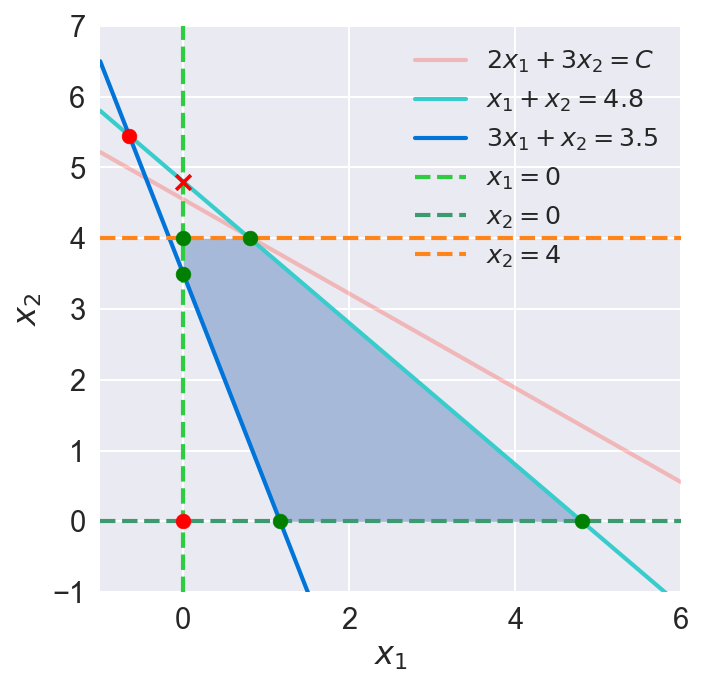
\includegraphics[scale=1]{system_2}
	\caption{Решение геометрическим методом}
	\label{pic:geometric_solution_2}
\end{center}
\end{figure}

Решим задачу двойственным симплекс методом. Добавим в таблице оптимального базиса 
\ref{tab:simplex_5} переменную $x_6$ к базисным переменным. Для этого выразим $x_6$ через свободные переменные $x_1$, $x_3$ и $x_5$:
\begin{equation*}
x_6 = 4 - x_2 = 4 - 4.8 + x_1 + x_3 = x_1 + x_3 - 0.8
\end{equation*}

Получившаяся симплекс таблица приведена в таблице \ref{tab:add_simplex_1}.

\begin{table}[H]
\begin{center}
	\def\tabcolsep{16pt}
	\def\arraystretch{1.3}
	\caption{Базис $x_2, x_4, x_6$}
	\label{tab:add_simplex_1}
	\begin{tabular}{|c||c|c|c||c|}
		\hline
		№1 & $x_1$ & $x_5$ & $x_3$ & $b$ \\ 
		\hhline{|=#===#=|}
		$x_4$ & $2$ & $1$ & $-1$ & $1.3$ \\ 
		\hline
		$x_2$ & $-1$ & $0$ & $-1$ & $4.8$\\  
		\hline
		$x_6$ & \textcolor{red}{\boldmath$1$} & $0$ & $1$ & $-0.8$\\ 
		\hhline{|=#===#=|}
		$f$ & $-1$ & $0$ & $-3$& $14.4$ \\ 
		\hline
	\end{tabular}
\end{center}
\end{table}

Так как $b \ngeqslant 0$, то базис является недопустимым. Выберем $x_1$ как разрешающий столбец, а $x_6$ как разрешающую строку. На их пересечении находится разрешающий элемент $1$. В таблице \ref{tab:add_simplex_2} приведена таблица симплекс метода, в которой поменяны местами $x_1$ и $x_6$.

\begin{table}[H]
\begin{center}
	\def\tabcolsep{16pt}
	\def\arraystretch{1.3}
	\caption{Базис $x_1, x_2, x_4$}
	\label{tab:add_simplex_2}
	\begin{tabular}{|c||c|c|c||c|}
		\hline
		№2 & $x_6$ & $x_5$ & $x_3$ & $b$ \\ 
		\hhline{|=#===#=|}
		$x_4$ & $2$ & $1$ & $-3$ & $2.9$ \\ 
		\hline
		$x_2$ & $-1$ & $0$ & $0$ & $4$\\  
		\hline
		$x_1$ & \textcolor{red}{\boldmath$1$} & $0$ & $-1$ & $0.8$\\ 
		\hhline{|=#===#=|}
		$f$ & $-1$ & $0$ & $-2$ & $13.6$ \\ 
		\hline
	\end{tabular}
\end{center}
\end{table}

Базис является допустимым, так как $b \ge 0$. Более того, базис является оптимальным, так как $c \leq 0$. Следовательно точка $x^{opt} = \begin{pmatrix} 0.8 & 4 & 0 & 0 & 2.9 & 0 \end{pmatrix}$ является оптимальным решением, что соотносится с геометрическим решением $x_1 = 0.8$, $x_2 = 4$. Значение функции в этой точке $f = 13.6$.

\section{Двойственная задача}

Сформулируем задачу, двойственную по отношению к исходной:

\begin{equation*}
\begin{cases}
	\max \left( 2 x_1 + 3 x_2 \right) \\
	x_1 + x_2 \le 4.8 \\
	-3 x_1 - x_2 \le -3.5 \\
	x_1 \ge 0 \\
	x_2 \ge 0
\end{cases}
\longleftrightarrow
\begin{cases}
	\min \left( 4.8 y_1 - 3.5 y_2 \right) \\
	y_1 - 3y_2 \ge 2 \\
	y_1 - y_2 \ge 3 \\
	y_1 \ge 0 \\
	y_2 \ge 0
\end{cases}
\end{equation*}

\end{document}